\documentclass[UTF8,a4paperdui, % draft
]{ctexart}
\usepackage[hidelinks]{hyperref}
\usepackage{bm}
\usepackage{graphicx}
\usepackage{pdfpages}
\usepackage{amsmath}
\usepackage{cite}
\usepackage{caption,subcaption}
\usepackage{geometry}
\usepackage{pdfpages}
\usepackage[ruled,vlined,boxed,linesnumbered]{algorithm2e}
\usepackage{listings}
\usepackage{color}
\lstset {
  basicstyle=\small\ttfamily,
  captionpos=b,
  tabsize=2,
  columns=fixed,
  breaklines=true,
  frame=l,
  numbers=left,
  numberstyle=\small\ttfamily,
  morekeywords= {
    EQUAL, GREATER, LESS, NONE, SOME, abstraction, abstype, and, andalso, array, as, before, bool, case, char, datatype, do, else, end, eqtype, exception, exn, false, fn, fun, functor, handle, if, in, include, infix, infixr, int, let, list, local, nil, nonfix, not, o, of, op, open, option, orelse, overload, print, raise, real, rec, ref, sharing, sig, signature, string, struct, structure, substring, then, true, type, unit, val, vector, where, while, with, withtype, word
  },
  morestring=[b]",
  morecomment=[s]{(*}{*)},
  stringstyle=\color{black},
  identifierstyle=\color{eclipseBlue},
  keywordstyle=\color{red},
  commentstyle=\color{eclipseGreen}
}
\definecolor{eclipseBlue}{RGB}{42,0.0,255}
\definecolor{eclipseGreen}{RGB}{63,127,95}


\geometry{left=4.0cm,right=4.0cm,top=5cm,bottom=5cm}
%%%%%%%%%%%%%%%%%%%%%%%%%%%%
%%%%%%%%%%%%%%%%%%%%%%%%%%%%
\DeclareMathOperator{\net}{net}
\DeclareMathOperator{\sups}{SuperString}
%%%%%%%%%%%%%%%%%%%%%%%%%%%%
%%%%%%%%%%%%%%%%%%%%%%%%%%%%

\makeatletter
\algocf@newcmdside@kobe{LetIn@let}{%
\KwSty{let}%
\ifArgumentEmpty{#1}\relax{ #1}%
\algocf@group{#2}%
\par
}
\algocf@newcmdside@kobe{LetIn@in}{%
\KwSty{in}%
\ifArgumentEmpty{#1}\relax{ #1}%
\algocf@block{#2}{end}{#3}%
\par
}
\newcommand\LetIn[2]{%
\LetIn@let{#1}%
\LetIn@in{#2}%
}
\makeatother

\newcommand\op{\texttt{op}}
\newcommand\ttt{\texttt}
\newcommand\tbf{\textbf}
\newcommand\tit{\textit}
\newcommand\tttt[1]{\text{\ttt{#1}}}
\newcommand\givepar[2]{\ttt{)}$^{#1\ #2}$\ttt{(}}
\usepackage{amssymb}
\usepackage{extarrows}
\begin{document}
\newpage
\newcommand*{\calF}{\mathcal{F}}
\newcommand*{\calH}{\mathcal{H}}
\newcommand*{\vx}{\bm x}
\newcommand*{\vy}{\bm y}
\newcommand*{\vh}{\bm h}
\newcommand{\Figure}[2]{
\begin{figure}[htbp]
\centering
\includegraphics[height=#1]{#2}
\end{figure}
}
%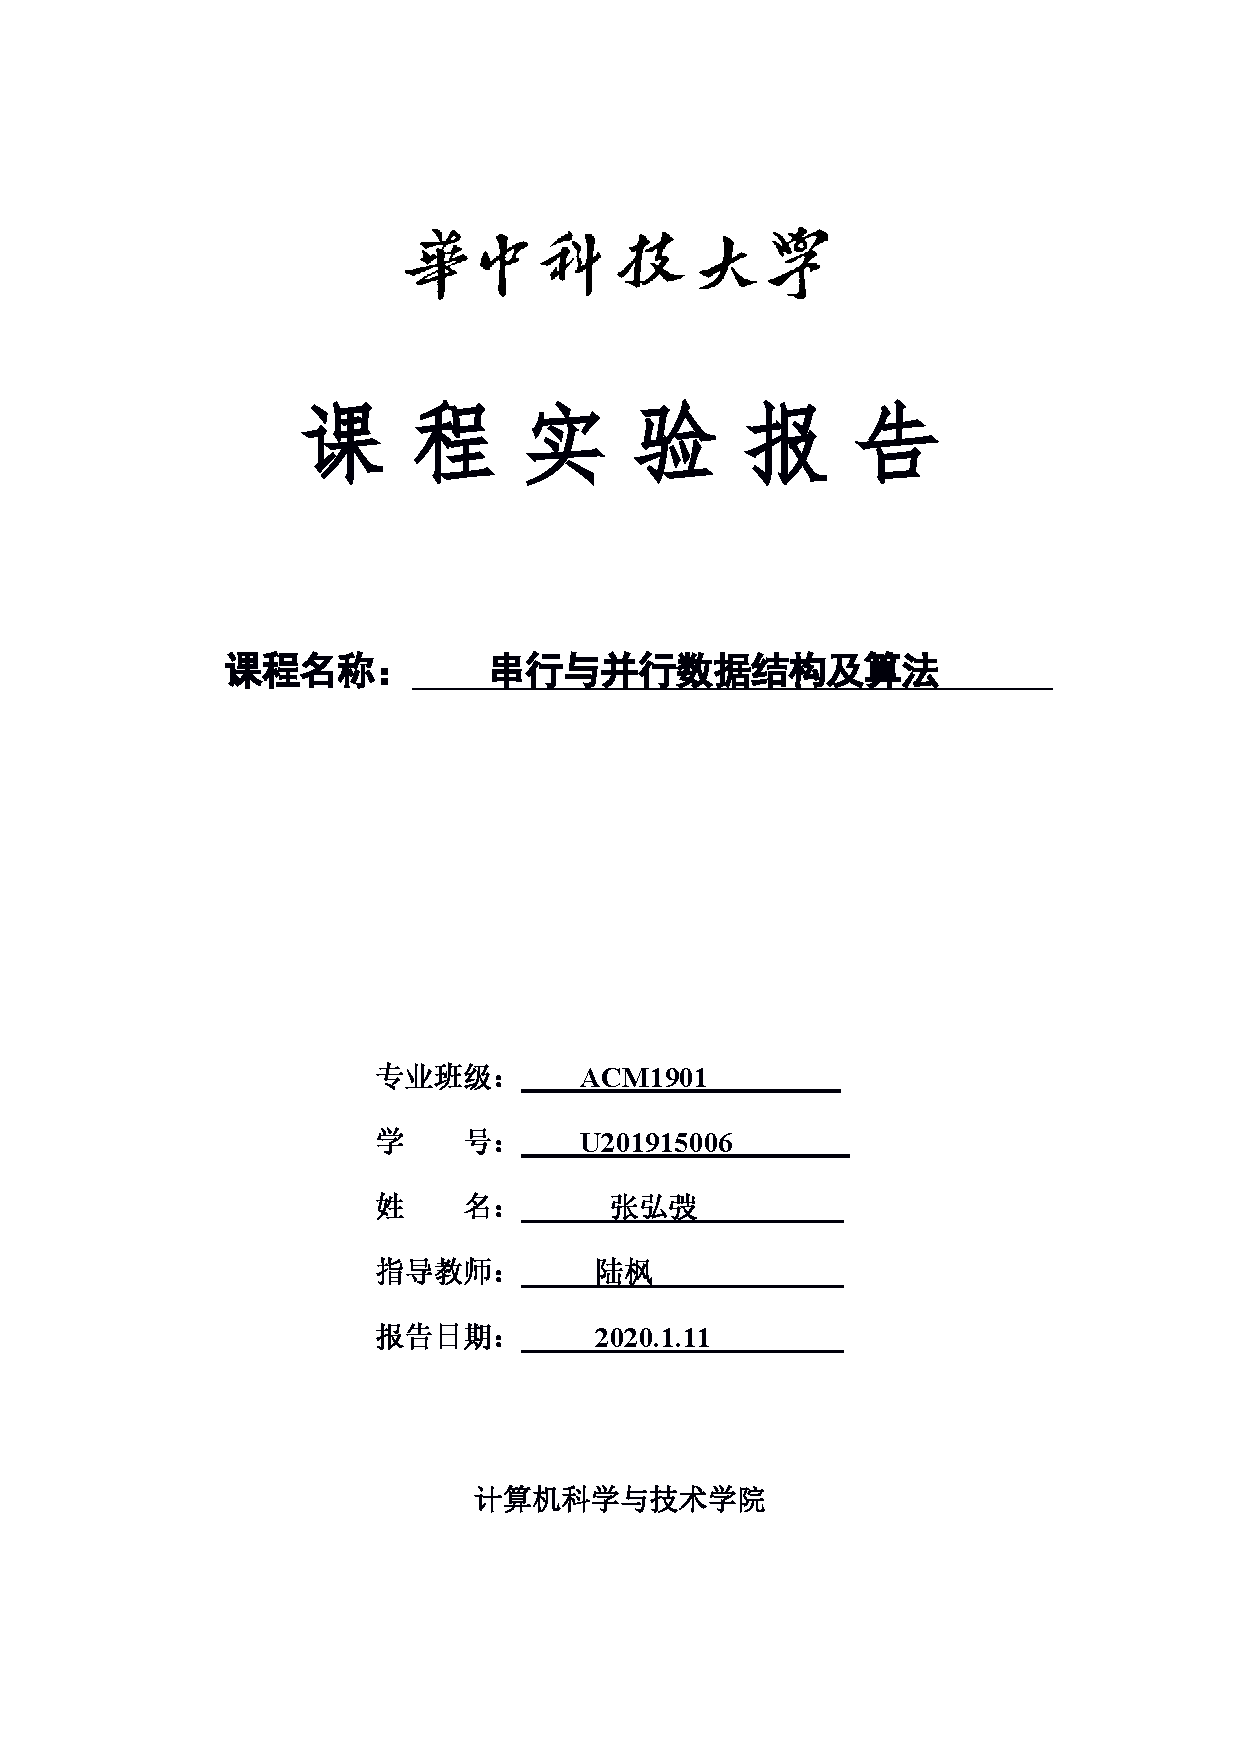
\includepdf{cover}
\tableofcontents
\newpage
\section{值的类型与输出}
\begin{lstlisting}
printInt(100);
printReal(3.5);
printString("Hello, world!");
\end{lstlisting}
\subsection{本关任务}
给出一个具有$N$个互不相同元素的数组,请对它进行升序排序。
\subsection{解法}
我们可以采用归并排序算法解决,即
\begin{algorithm}
\SetAlgoLined
MergeSort($\langle a_n\rangle$) =\par
\eIf{$|a_n|=1$}{$a_1$}{
\LetIn{
$L\longleftarrow $ MergeSort($\langle a_1,\ a_2,\ \ldots,\ a_{(n+1)/2}\rangle$)\;
$R\longleftarrow $ MergeSort($\langle a_{(n+1)/2},\ \ldots,\ a_{n}\rangle$)\;
}{
Merge($L, R$)}}
\caption{MergeSort}
\end{algorithm}\\
复杂度为
\[
W=O(n\log n)\quad S=O(\log^2n)
\]

\section{更大的斐波那契数列}
\subsection{本关任务}
编写一个能计算任意大小斐波那契数列的程序。
\subsection{解法}
可以采用矩阵快速幂的方法快速计算斐波那契序列。
\begin{algorithm}
\SetAlgoLined
Fibonacci($n$) =\par
\LetIn{
$e\longleftarrow $[[1,1],[0,1]]\par
$f(n,\ e)=$\par
\eIf{$(n=1)$}{$e$}{\eIf{$n\ mod\ 2\ =\ 0$}{$f(n\ div\ 2,\ e\cdot e $)}{$e\cdot f((n-1)\ div\ 2,\ e\cdot e)$}}}
{$List.nth(f(n)\cdot [1,0],\ 1)$}
\caption{quickFibonacci}
\end{algorithm}\\
为计算第$n$个斐波那契数,从基础矩阵$e\ =\ [[1,1],[0,1]]$开始,若$n$为大于1的偶数,则将$e$更新为$e\cdot e$并将$n$整除$2$;若$n$为大于1的奇数,则在该步骤的返回值乘以$e$并更新参数$e\ =e\ \cdot e$,$n\ =\ n\ div\ 2$。直到$n$为1,则返回返回$f$中的第二个参数。
\subsection{分析与证明}
实现斐波那契数列的快速运算的矩阵快速幂用到的基础矩阵是[[1,1],[0,1]]的二阶矩阵。\\
计算第$n$个数需要计算$\lceil logn\rceil$次,因此$W$为$logn$。由于无法并行运算,所以$S=logn$。



\section{二分查找}
\subsection{本关任务}
给定一个长为$N$的递增序列,以及$Q$次查询,从这个序列里查找一些数是否存在。
\subsection{解法}
可以采用矩阵快速幂的方法快速计算斐波那契序列。
\begin{algorithm}
\SetAlgoLined
Fibonacci($n$) =\par
\LetIn{
$e\longleftarrow $[[1,1],[0,1]]\par
$f(n,\ e)=$\par
\eIf{$(n=1)$}{$e$}{\eIf{$n\ mod\ 2\ =\ 0$}{$f(n\ div\ 2,\ e\cdot e $)}{$e\cdot f((n-1)\ div\ 2,\ e\cdot e)$}}}
{$List.nth(f(n)\cdot [1,0],\ 1)$}
\caption{quickFibonacci}
\end{algorithm}\\
为计算第$n$个斐波那契数,从基础矩阵$e\ =\ [[1,1],[0,1]]$开始,若$n$为大于1的偶数,则将$e$更新为$e\cdot e$并将$n$整除$2$;若$n$为大于1的奇数,则在该步骤的返回值乘以$e$并更新参数$e\ =e\ \cdot e$,$n\ =\ n\ div\ 2$。直到$n$为1,则返回返回$f$中的第二个参数。
\subsection{分析与证明}
实现斐波那契数列的快速运算的矩阵快速幂用到的基础矩阵是[[1,1],[0,1]]的二阶矩阵。\\
计算第$n$个数需要计算$\lceil logn\rceil$次,因此$W$为$logn$。由于无法并行运算,所以$S=logn$。

\section{无重复排序}
\subsection{本关任务}
给出一个具有$N$个互不相同元素的数组,请对它进行升序排序。
\subsection{解法}
我们可以采用归并排序算法解决,即
\begin{algorithm}
\SetAlgoLined
MergeSort($\langle a_n\rangle$) =\par
\eIf{$|a_n|=1$}{$a_1$}{
\LetIn{
$L\longleftarrow $ MergeSort($\langle a_1,\ a_2,\ \ldots,\ a_{(n+1)/2}\rangle$)\;
$R\longleftarrow $ MergeSort($\langle a_{(n+1)/2},\ \ldots,\ a_{n}\rangle$)\;
}{
Merge($L, R$)}}
\caption{MergeSort}
\end{algorithm}\\
复杂度为
\[
W=O(n\log n)\quad S=O(\log^2n)
\]

\end{document}
